\begin{figure}[htbp]
\centering
\begin{tikzpicture}[font=\small]
\node[anchor=east] at (-.2,1.1) {original class:};
\node[draw,rounded corners,minimum width=2.2cm] (ordinary) at (1.3,1.1)
 {$q-4$ other lines};
\node[draw,rounded corners,minimum width=2.2cm] (merged) at (4.1,1.1)
 {$M_g^0,\ M_g^1$};
\node[draw,rounded corners,minimum width=2.2cm] (split) at (6.9,1.1)
 {$S_g^1,\ S_g^2$};
\node[anchor=east] at (-.2,0) {new blocks:};
\node[draw,rounded corners,minimum width=2.2cm] (ordinary2) at (1.3,0)
 {$q-4$ blocks};
\node[draw,rounded corners,minimum width=2.2cm] (merged2) at (4.1,0)
 {$1$ merged block};
\node[draw,rounded corners,minimum width=2.2cm] (split2) at (6.9,0)
 {$4$ pair blocks};
\draw[-{Stealth}] (ordinary)--(ordinary2);
\draw[-{Stealth}] (merged)--(merged2);
\draw[-{Stealth}] (split)--(split2);
\end{tikzpicture}

\medskip
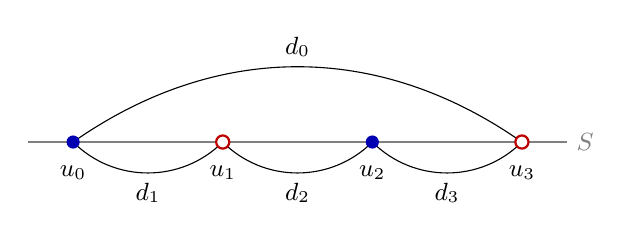
\begin{tikzpicture}[scale=.95,font=\small]
\draw[gray] (-.6,0)--(6.6,0) node[right] {$S$};
\foreach \i/\x in {0/0,1/2,2/4,3/6}{
 \coordinate (u\i) at (\x,0);
 \node[below=5pt] at (u\i) {$u_\i$};}
\draw (u0) to[bend right=45] node[below] {$d_1$} (u1);
\draw (u1) to[bend right=45] node[below] {$d_2$} (u2);
\draw (u2) to[bend right=45] node[below] {$d_3$} (u3);
\draw (u3) to[bend right=35] node[above] {$d_0$} (u0);
\foreach \i in {0,2}{\fill[blue!70!black] (u\i) circle (2.5pt);}
\foreach \i in {1,3}{\draw[red!75!black,thick,fill=white] (u\i) circle (2.5pt);}
\end{tikzpicture}
\caption{The merge and split operation gives $q+1$ blocks per direction.
Below, the four points on one split line form two opposite-pair blocks,
shown by filled and open points. An arc labelled $d_i$ means that its
endpoints lie on different constituents of the merged pair in direction
$d_i$, and hence share its block label. The arcs record this relation;
they are not affine lines. The diagram is schematic.}
\label{fig:cycle}
\end{figure}
